\documentclass{article}

\usepackage[T1]{fontenc}
\usepackage[utf8]{inputenc}
\usepackage{graphicx}
\usepackage{caption}
\usepackage[font=small,labelfont=bf]{caption}
\usepackage{booktabs, siunitx}
\usepackage{tikz}
\usepackage{tikz-qtree}
\usepackage{pifont}
\usepackage[margin=0.90in]{geometry}
\usepackage{etoolbox,titling}
\usepackage{enumitem}
\usepackage{fancyhdr}
\usepackage{soulutf8}
\usepackage{epigraph}
\usepackage{amssymb}
\usepackage{amsmath}

\pagestyle{fancy}
\fancyhf{}
\rhead{Chiara Solito}
\lhead{Dispense di Laboratorio di Bioinformatica}
\rfoot{Pagina \thepage}
\lfoot{Bioinformatica - A.A. 2021/22}
\usetikzlibrary{trees}
\tikzstyle{every node}=[draw=black,thick,anchor=west]
\newcommand{\angstrom}{\mbox{\normalfont\AA}}

\begin{document}
\newcommand\tab[1][0.3cm]{\hspace*{#1}}


\begin{titlepage}
    \begin{center}
        \vspace*{1cm}
            
        \Huge
        \textbf{Vaccine Supervision}
            
        \vspace{0.5cm}
        \LARGE
        Progetto di Ingegneria del Software
            
        \vspace{1.5cm}
            
        \textbf{Virginia Filippi e Chiara Solito}

        \vspace{0.8cm}

            
        \Large
        Corso di Laurea in Bioinformatica\\
        Università degli studi di Verona\\
        A.A. 2021/22
            
    \end{center}
\end{titlepage}
La presente è la documentazione blablabla.\\
Insieme a questo documento in formato PDF viene fornito anche il codice \LaTeX  con cui è stato generato.
\tableofcontents
\thispagestyle{empty}
\newpage
\thispagestyle{empty}

\section{Traccia dell'Elaborato}
\section{Analisi e Specifica dei Requisiti}
(\dots )\\
\subsection{Specifiche casi d'uso}
In questa sezione definiamo le proprietà dell'applicazione.\\
Come dichiarato nella traccia il sistema prevede l'utilizzo da parte di due tipologie di personale medico: Medico e Farmacologo. 
Entrambi i tipi di utente possono utilizzare l'applicazione dopo opportuno login: in questa sede si è previsto che gli utenti siano pre-registrati da un amministratore di sistema esterno (sul modello di sistemi medici già noti). Non è stato quindi previsto un form di registrazione, durante lo sviluppo.
\begin{figure}[htp]
    \centering
    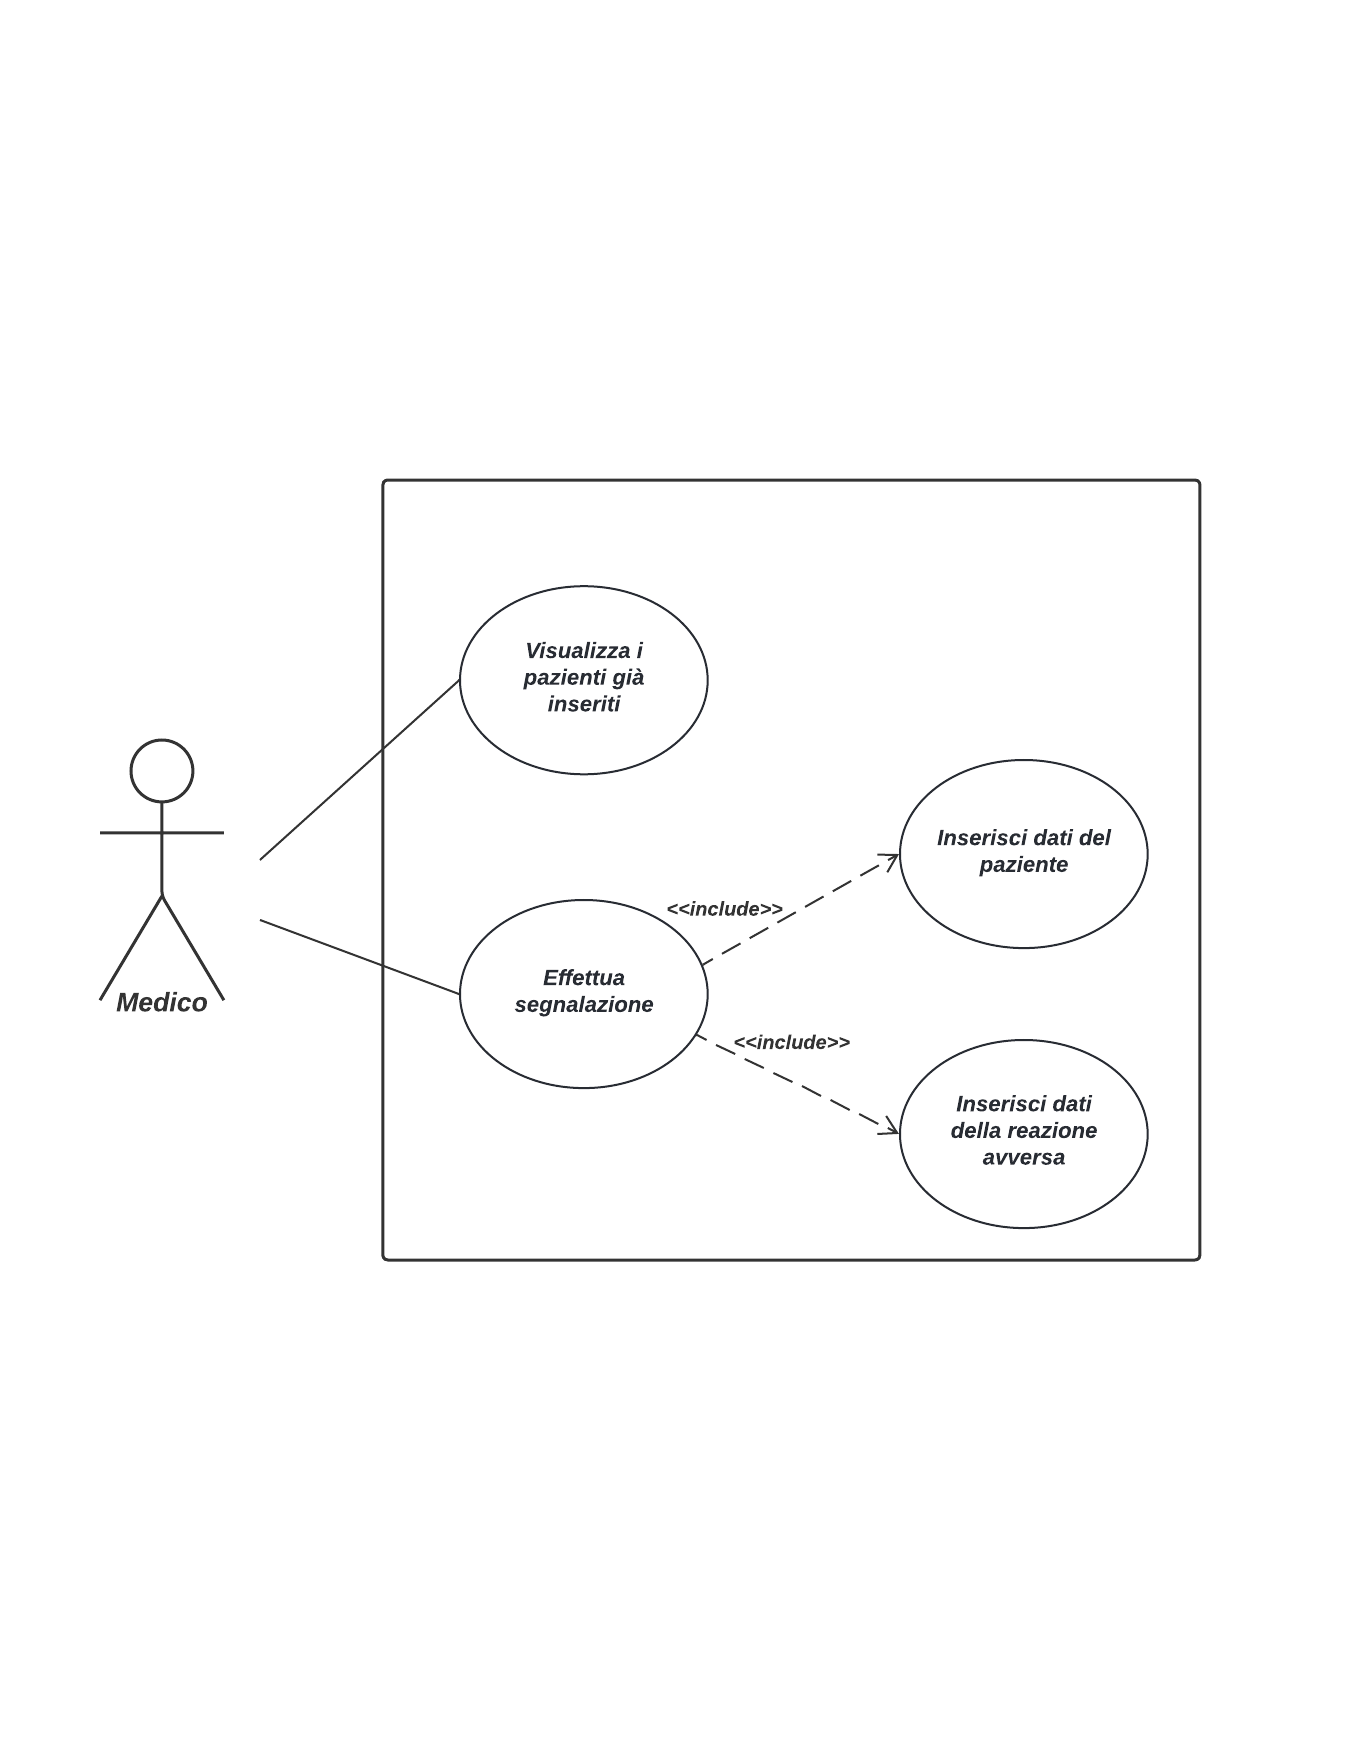
\includegraphics[width=0.7\textwidth]{pictures/CasoDUsoMedico_SfondoTrasparente.png}
    \caption{Caso d'uso Medico}
\end{figure}
\section{Implementazione del DataBase}
Come richiesto dalla traccia si è implementato un database con cui l'applicazione potesse interagire.\\
Il Database è stato creato sulla base dell'ER qui riportato:
\begin{figure}[h]
    \centering
    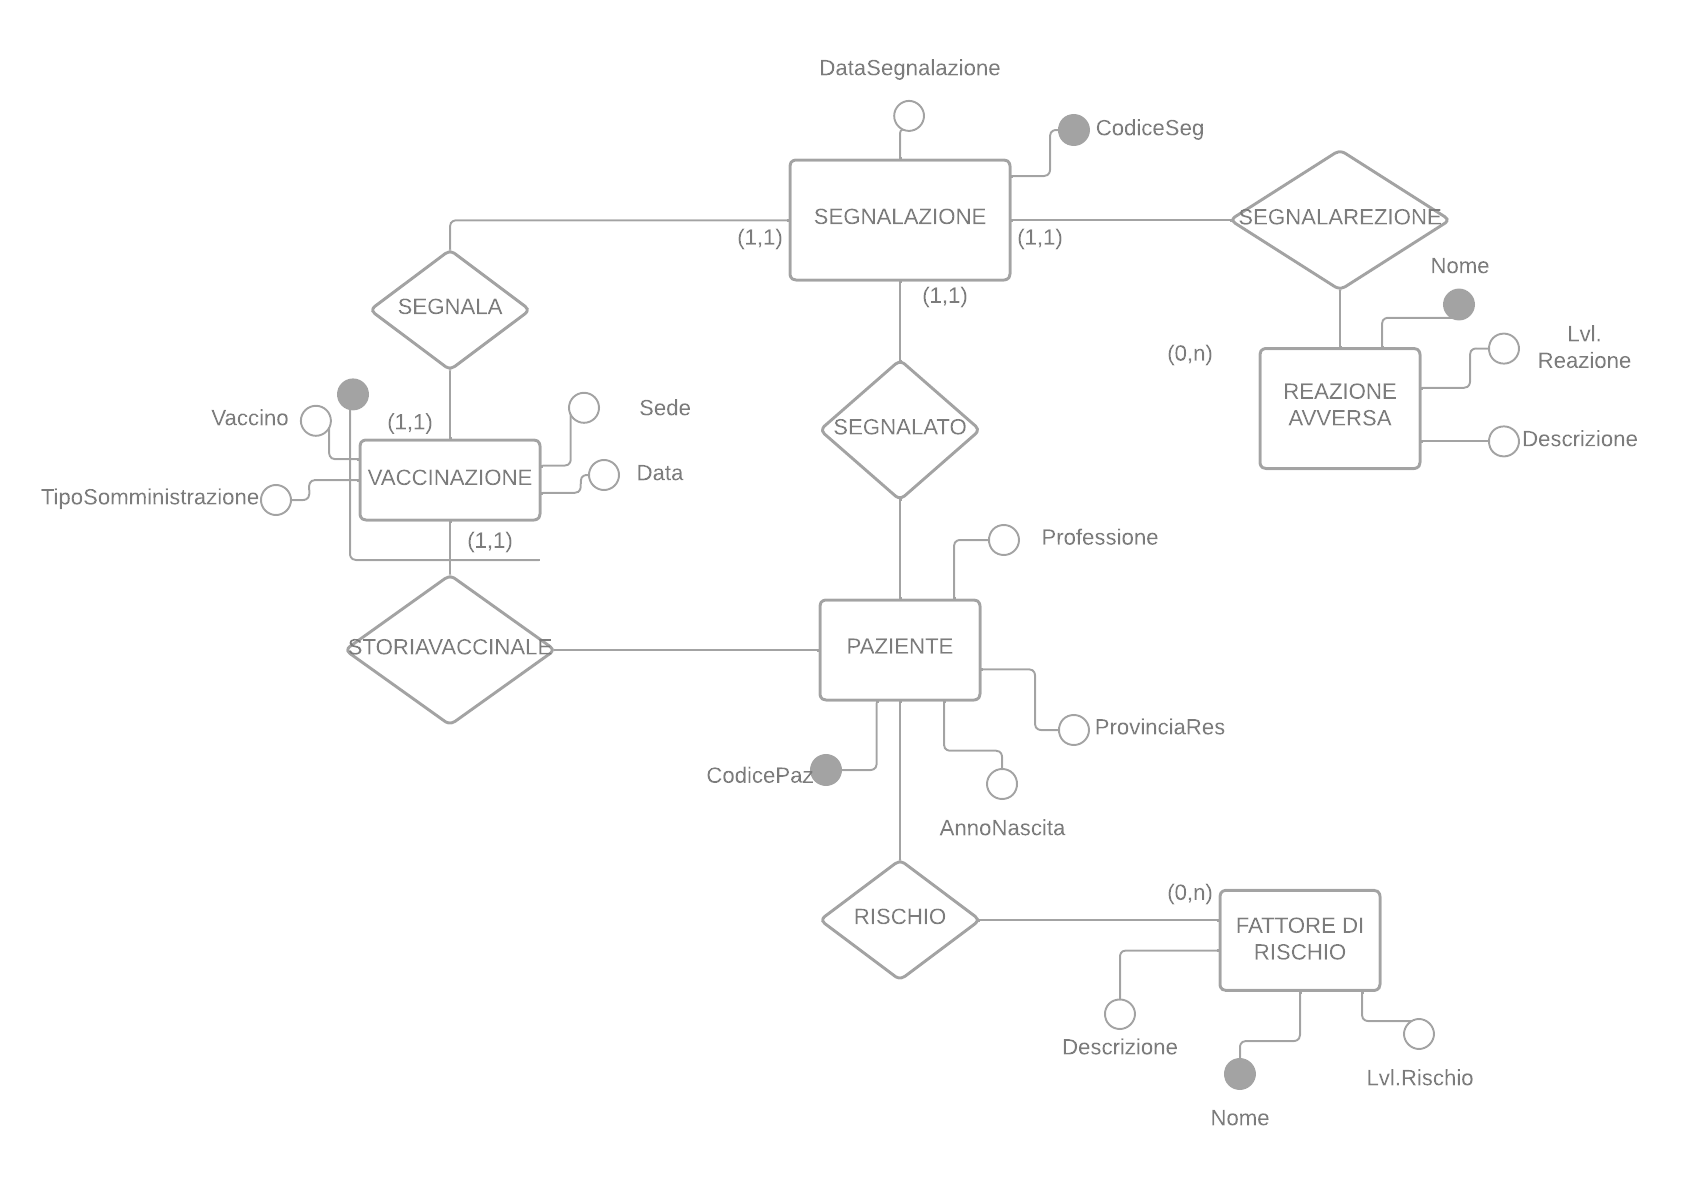
\includegraphics[width=0.7\textwidth]{pictures/_Diagramma vuoto.png}
    \caption{Da modificare!!!}
\end{figure}
Si è scelto di implementare il Database in PostgreSQL. Riportiamo anche le query usate per la creazione delle tabelle, che ci aiutano a comprendere com'è fatto:
\paragraph*{Tabella PAZIENTE}
\begin{verbatim}
    CREATE TABLE Paziente(
        codice SERIAL PRIMARY KEY,
        annonascita NUMERIC(4) NOT NULL ,
        CHECK ( annonascita >= 1900 ),
        provincia VARCHAR(20) NOT NULL,
        professione VARCHAR(20) NOT NULL
    );
\end{verbatim}
\paragraph*{Tabella FATTORERISCHIO}
\begin{verbatim}
    CREATE TABLE FattoreRischio(
        nome VARCHAR(20) PRIMARY KEY,
        descrizione VARCHAR(50),
        lvlrischio NUMERIC(1) NOT NULL,
        CHECK ( lvlrischio >= 1 AND lvlrischio <= 5 )
    );
\end{verbatim}
\paragraph*{Tabella VACCINAZIONE}
\begin{verbatim}
    CREATE TABLE Vaccinazione(
        pazienteID INTEGER REFERENCES paziente(codice),
        vaccino VARCHAR(15) NOT NULL,
        tiposomministrazione VARCHAR(10) NOT NULL,
        PRIMARY KEY (pazienteID, vaccino, tiposomministrazione),
        sedevaccino VARCHAR(10) NOT NULL,
        datavaccino DATE NOT NULL
    );
\end{verbatim}
\paragraph*{Tabella REAZIONEAVVERSA}
\begin{verbatim}
    CREATE TABLE ReazioneAvversa(
        nome VARCHAR(20) PRIMARY KEY,
        gravita NUMERIC(1) NOT NULL,
        CHECK(gravita >= 1 AND gravita <= 5),
        descrizione VARCHAR(50) NOT NULL
    );
\end{verbatim}
\paragraph*{Tabella SEGNALAZIONE}
\begin{verbatim}
    CREATE TABLE Segnalazione(
        codice SERIAL PRIMARY KEY,
        datareazione DATE NOT NULL,
        datasegnalazione DATE NOT NULL DEFAULT CURRENT_DATE,
        reazione VARCHAR(20) NOT NULL REFERENCES reazioneavversa(nome),
        pazienteID INTEGER NOT NULL,
        vaccino VARCHAR(15) NOT NULL,
        tiposomm VARCHAR(10) NOT NULL,
        FOREIGN KEY(pazienteID, vaccino, tiposomm) 
            REFERENCES vaccinazione(pazienteid, vaccino, tiposomministrazione)
    );
\end{verbatim}
\paragraph*{Tabella RISCHIOPAZIENTE}
\begin{verbatim}
    CREATE TABLE RischioPaziente(
        pazienteID INTEGER NOT NULL REFERENCES paziente(codice),
        rischio VARCHAR(20) NOT NULL REFERENCES fattorerischio(nome),
        PRIMARY KEY(pazienteID, rischio)
    );
\end{verbatim}
\end{document}